\documentclass[border=5]{standalone}
\usepackage{calculator}
\usepackage{tikz}
\usetikzlibrary{arrows, arrows.meta, positioning}

\tikzset{    
    disk/.style={ thick },
    traj/.style={ thin, dashed, -Latex },
    point/.style={ color=black, circle, scale=0.3, fill },
    partition/.style={ right, scale=0.75 },
    label/.style={ scale=0.5, black, below = 0.5mm },
    time/.style={ scale=0.75, above left }
}

\definecolor{light-gray}{gray}{0.45}

\def\xMin{0}
\def\xMax{3}
\def\yMin{0}
\def\yMax{3}
\def\xWidth{1.5}
\def\oPacity{0.75}
\def\ySlant{0.5}
\def\xSlant{-0.9}
\def\z{50}
\def\speed{0.2}
\def\R{0.05}

\newcommand{\drawFrame}[3]{
    \fill[orange, opacity=0.65] (#1*\xWidth-#3,#1*\xWidth-#3) rectangle (#2*\xWidth+#3,#2*\xWidth+#3);
    \draw[black!70] (#1*\xWidth-#3,#1*\xWidth-#3) rectangle (#2*\xWidth+#3,#2*\xWidth+#3);
}

\newcommand{\drawWhiteFrameA}[3]{
    \fill[white, opacity=0.75] (#1*\xWidth-#3,#1*\xWidth-#3) rectangle (#2*\xWidth+#3,#2*\xWidth+#3);
    \draw[black, dashed, opacity=0.75] (#1*\xWidth-#3,#1*\xWidth-#3) rectangle (#2*\xWidth+#3,#2*\xWidth+#3);
}

\newcommand{\drawBlueFrame}[5]{
    \fill[blue, opacity=0.5] (#1*\xWidth-#5,#2*\xWidth-#5) rectangle (#3*\xWidth+#5,#4*\xWidth+#5);
    \draw[black!70] (#1*\xWidth-#5,#2*\xWidth-#5) rectangle (#3*\xWidth+#5,#4*\xWidth+#5);
}

\newcommand{\drawWhiteFrameB}[5]{
    \fill[white, opacity=0.75] (#1*\xWidth-#5,#2*\xWidth-#5) rectangle (#3*\xWidth+#5,#4*\xWidth+#5);
    \draw[black, dashed, opacity=0.75] (#1*\xWidth-#5,#2*\xWidth-#5) rectangle (#3*\xWidth+#5,#4*\xWidth+#5);
}

\newcommand{\drawFlocks}[1]{
    \draw [fill=lime   ](A#1) circle (\R) ;
    \draw [fill=magenta](B#1) circle (\R) ;
    \draw [fill=teal](C#1) circle (\R) ;
}

\newcommand{\drawLabels}[1]{
    \node[label] at (A#1) {$a$};
    \node[label] at (B#1) {$b$};
    \node[label] at (C#1) {$c$};
}

\newcommand{\drawTrajs}[1]{
        \def\i{}
        \ADD{#1}{-1}{\i}
        \draw[traj] (A\i) -- (A#1);
        \draw[traj] (B\i) -- (B#1);
        \draw[traj] (C\i) -- (C#1);
}

\begin{document}
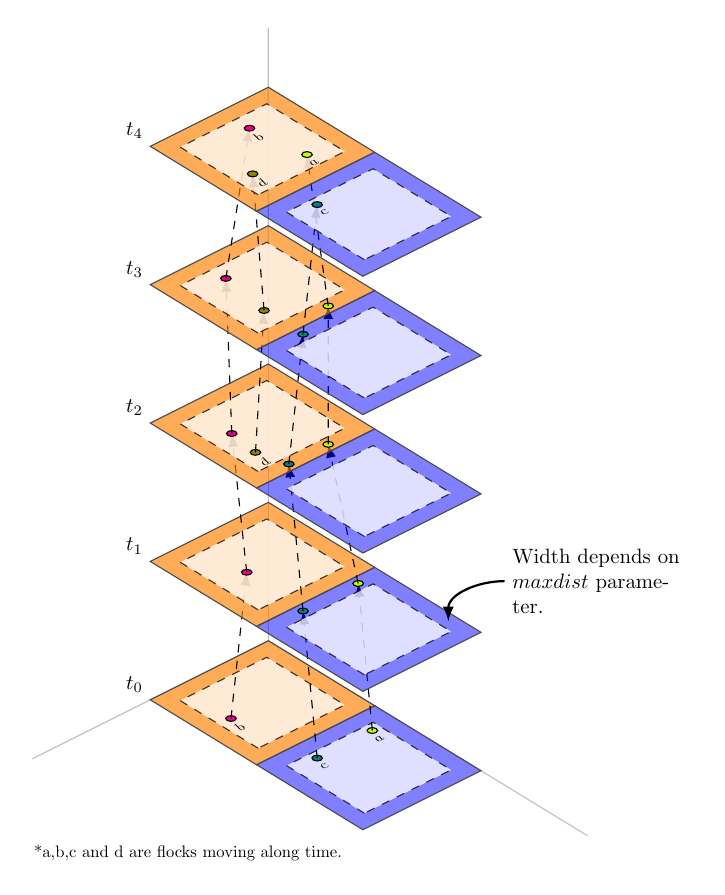
\begin{tikzpicture}    
    \draw[] (-2.75,0.45) node[scale=0.6,right]{*a,b,c and d are flocks moving along time.};
    \def\t{0};
    \begin{scope}
        [yshift=0*\z, every node/.append style={yslant=\ySlant,xslant=\xSlant},yslant=\ySlant,xslant=\xSlant]
        \coordinate (O) at (3,3);
        \coordinate (T) at (\xMin+1.5, \xMax);
        \coordinate (A\t) at (2.70, 1.20);
        \coordinate (B\t) at (1.85, 2.25);
        \coordinate (C\t) at (2.00, 1.20);

        \draw[black!25] (O) -- (3,-1.5);
        \draw[black!25] (O) -- (0,3);
        \draw[black!25] (O) -- (10,10.78);
        \drawFrame{1}{2}{0*\speed};
        \drawBlueFrame{1}{0}{2}{1}{\t*\speed};
        \drawWhiteFrameA{1}{2}{-1*\speed};
        \drawWhiteFrameB{1}{0}{2}{1}{-1*\speed};
        \drawFlocks{0}
        \drawLabels{0}
    \end{scope}
    \node[time] at (T) {$t_\t$};

    \def\t{1};
    \begin{scope}
        [yshift=1*\z, every node/.append style={yslant=\ySlant,xslant=\xSlant},yslant=\ySlant,xslant=\xSlant]
        \coordinate (T) at (\xMin+1.5, \xMax);
        \coordinate (InfoPointer) at (2.9,0.35);\coordinate (InfoText) at (3.75,0.5);
        \coordinate (A\t) at (2.70, 1.40);
        \coordinate (B\t) at (2.05, 2.25);
        \coordinate (C\t) at (2.00, 1.40);

        \drawTrajs{1}
        \drawFrame{1}{2}{0*\speed};
        \drawBlueFrame{1}{0}{2}{1}{0*\speed};
        \drawWhiteFrameA{1}{2}{-1*\speed};
        \drawWhiteFrameB{1}{0}{2}{1}{-1*\speed};
        \drawFlocks{1}
    \end{scope}
    \node[time] at (T) {$t_\t$};
    \draw[-latex,thick] (InfoText) node[scale=0.75,right,text width=3cm]{Width depends on $maxdist$ parameter.} to[out=180,in=90] (InfoPointer);
    
    \def\t{2};
    \begin{scope}
        [yshift=2*\z, every node/.append style={yslant=\ySlant,xslant=\xSlant},yslant=\ySlant,xslant=\xSlant]
        \coordinate (T) at (\xMin+1.5, \xMax);
        \coordinate (A\t) at (2.50, 1.60);
        \coordinate (B\t) at (1.95, 2.35);
        \coordinate (C\t) at (2.00, 1.60);
        \coordinate (D\t) at (1.90, 1.96);

        \drawTrajs{2}
        \drawFrame{1}{2}{0*\speed};
        \drawBlueFrame{1}{0}{2}{1}{0*\speed};
        \drawWhiteFrameA{1}{2}{-1*\speed};
        \drawWhiteFrameB{1}{0}{2}{1}{-1*\speed};
        \drawFlocks{2}
        \draw [fill=olive](D\t) circle (\R) ;
        \node[label] at (D\t) {$d$};
    \end{scope}
    \node[time] at (T) {$t_\t$};

    \def\t{3};
    \begin{scope}
        [yshift=3*\z, every node/.append style={yslant=\ySlant,xslant=\xSlant},yslant=\ySlant,xslant=\xSlant]
        \coordinate (T) at (\xMin+1.5, \xMax);
        \coordinate (A\t) at (2.50, 1.60);
        \coordinate (B\t) at (2.1, 2.6);
        \coordinate (C\t) at (2.00, 1.40);
        \coordinate (D\t) at (2.00, 1.95);

        \drawTrajs{3}
        \def\i{};\ADD{\t}{-1}{\i};
        \draw[traj] (D\i) -- (D\t);
        \drawFrame{1}{2}{0*\speed};
        \drawBlueFrame{1}{0}{2}{1}{0*\speed};
        \drawWhiteFrameA{1}{2}{-1*\speed};
        \drawWhiteFrameB{1}{0}{2}{1}{-1*\speed};
        \drawFlocks{3}
        \draw [fill=olive](D\t) circle (\R) ;
    \end{scope}
    \node[time] at (T) {$t_\t$};
    
    \def\t{4};
    \begin{scope}
        [yshift=4*\z, every node/.append style={yslant=\ySlant,xslant=\xSlant},yslant=\ySlant,xslant=\xSlant]
        \coordinate (T) at (\xMin+1.5, \xMax);
        \coordinate (A\t) at (2.5, 1.90);
        \coordinate (B\t) at (2.4, 2.6);
        \coordinate (C\t) at (2.00, 1.20);
        \coordinate (D\t) at (1.90, 2);

        \drawTrajs{4}
        \def\i{};\ADD{\t}{-1}{\i};
        \draw[traj] (D\i) -- (D\t);
        \drawFrame{1}{2}{0*\speed};
        \drawBlueFrame{1}{0}{2}{1}{0*\speed};
        \drawWhiteFrameA{1}{2}{-1*\speed};
        \drawWhiteFrameB{1}{0}{2}{1}{-1*\speed};
        \drawFlocks{4}
        \draw [fill=olive](D\t) circle (\R) ;
        \node[label] at (A\t) {$a$};
        \node[label] at (B\t) {$b$};
        \node[label] at (C\t) {$c$};
        \node[label] at (D\t) {$d$};
    \end{scope}
    \node[time] at (T) {$t_\t$};
\end{tikzpicture}
\end{document} 
